\chapter{Image Processing and NDVI}
\label{sec:image_processing}
SIFT, mapping, geotagging, alignment,\\

Once the images are undistorted as in section \ref{sec:undistortion}, the images can be aligned using stereo-correspondence before an NDVI is performed.

A scale-invariant-feature-transform is applied to the images to align them using an affine transform. An NDVI calculation is applied to the matched images, with a floating point output image. A LUT colourmap is applied to visibly distinguish different areas and their meanings in the final image.

\section{Feature Detection}

There are different types of feature detection. 
\begin{itemize}
	\item Harris Corner Detection
	\item Shi-Tomasi Corner Detection
	\item SIFT (Scale-Invariant Feature Transform)
	\item SURF (Speeded-Up Robust Features)
	\item FAST (Features from Accelerated Segment Test)
	\item BRIEF (Binary Robust Independent Elementary Features)
	\item ORB (Oriented FAST and Rotated BRIEF)
	\item BRISK, FREAK, KAZE, and AKAZE
\end{itemize}

There are also different types of feature matching.

\begin{itemize}
	\item Feature Matching + Homography to find Objects
	\item FLANN (Fast Library for Approximate Nearest Neighbors) based matcher
\end{itemize}

Harris Corner detection is useful for the chessboard calibration technique as in section \ref{sec:cal_technique}. Shi-Tomasi improved the scoring function of Harris, but it is more appropriate for tracking. SIFT provides keypoints and descriptors. It also does not depend on the scale of a corner, unlike in Figure \ref{fig:sift_scale}. SURF is good at dealing with blurring and rotation, but not at handling viewpoint and illumination change as in SURF. FAST is better from a realtime, limited resource application point of view. Although it is several times faster than the other detectors, it is not robust against high levels of noise, and depends on a threshold. BRIEF is a quicker feature descriptor with lower memory usage, but feature detection such as SIFT, SURF is still needed. ORB is a good alternative to SIFT and SURF in performance, and is not patented.\\

\begin{figure}[H]
\centering
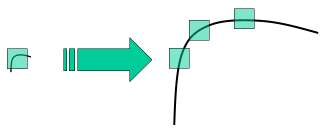
\includegraphics[scale=0.5]{images/sift_scale_invariant.jpg}
\caption{Harris corner detection on scaled corners. \cite{calib3d}}
\label{fig:sift_scale}
\end{figure}

\subsection{Feature matching}
Brute-force feature matching calculates the distance between a descriptor in the first set and all the features in the second set, returning the closest one.

%SURF is faster than SIFT, since it approximates the Laplacian of Gaussian with Box Filter instead of Difference of Gaussian.

\subsection{Homography}



\section{Stitching and mapping}

A few images are stitched together to show proof-of-concept as in Figure \ref{fig:stitch_map}.

\begin{figure}[H]
\centering
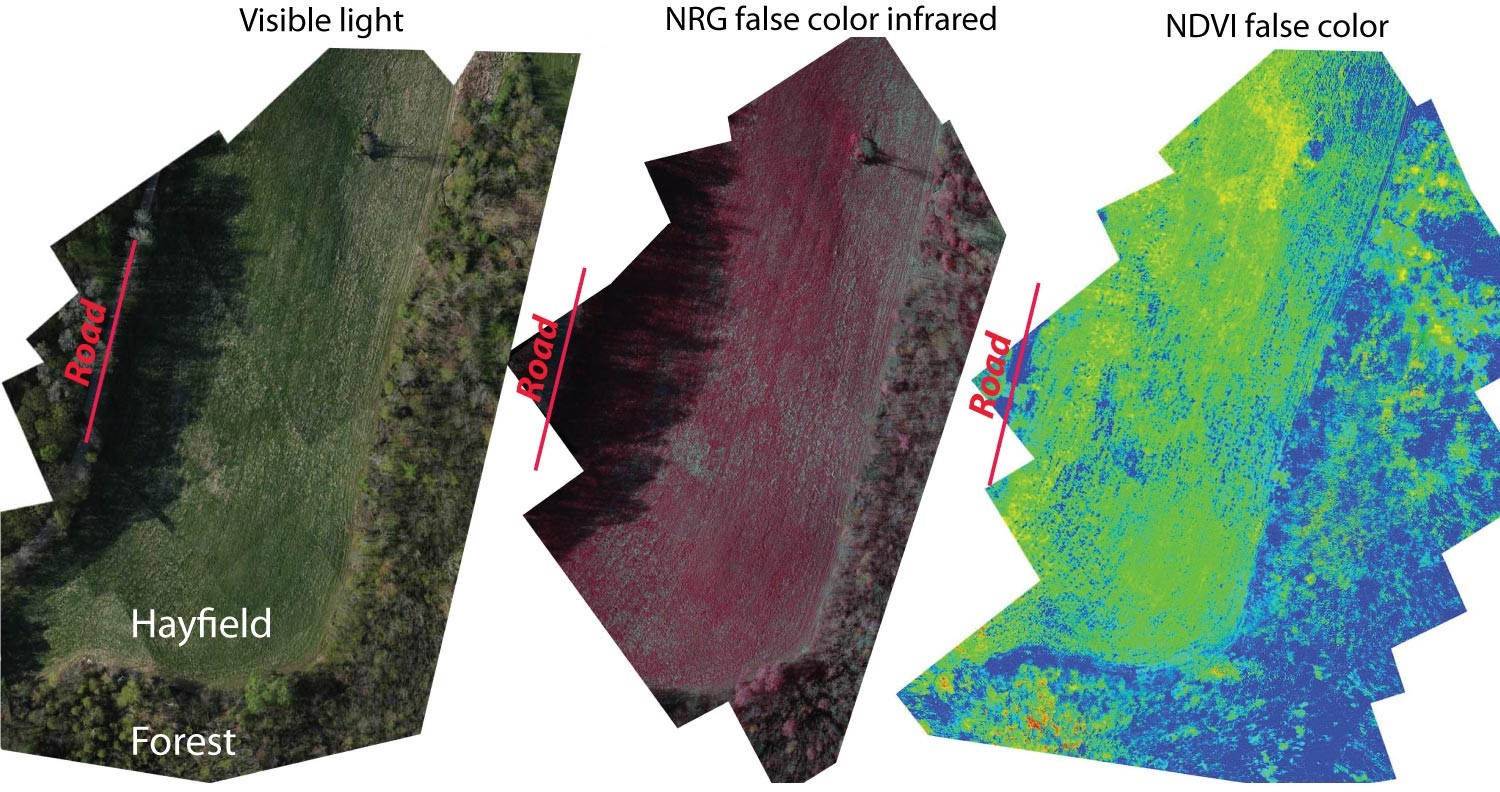
\includegraphics[scale=0.35]{images/ndvi_stitch_example.jpg}
\caption{Photos stitched into a map}
\label{fig:stitch_map}
\end{figure}

\section{Calibration Plate}

\begin{figure}[H]
\begin{subfigure}{0.5\textwidth}
\centering
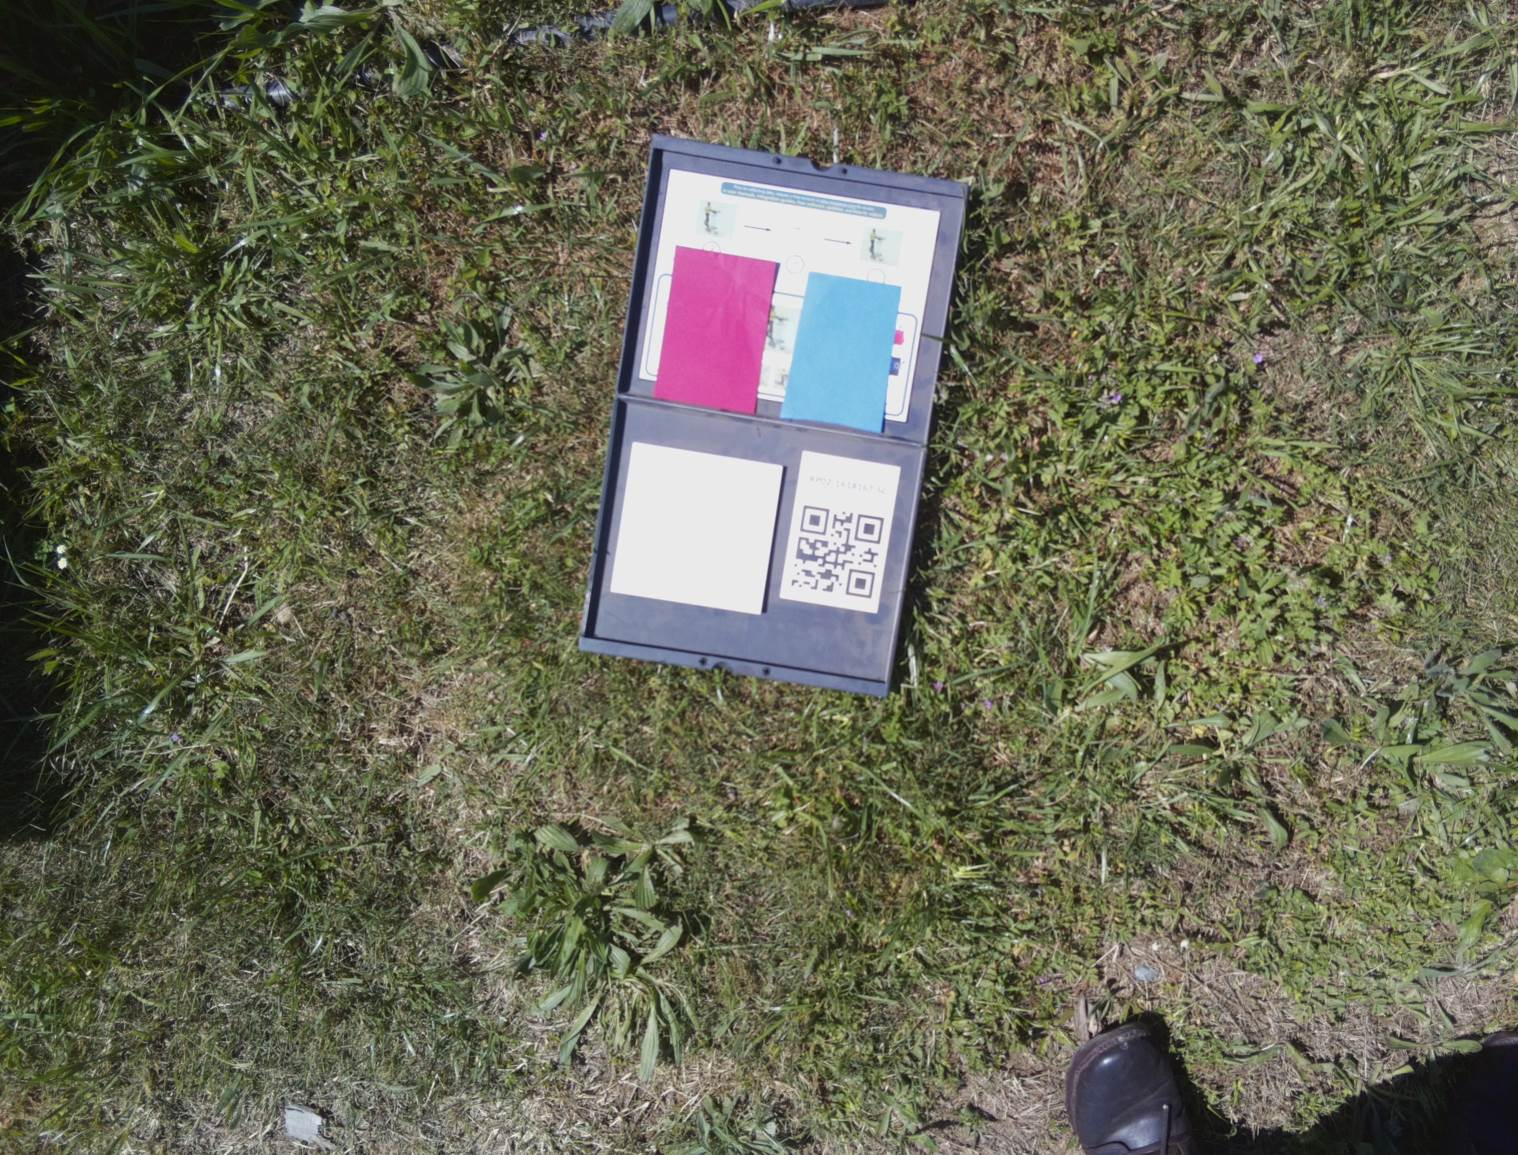
\includegraphics[scale=0.17]{images/rgb_cal.jpg}
\caption{RGB image}
\end{subfigure}
\begin{subfigure}{0.5\textwidth}
\centering
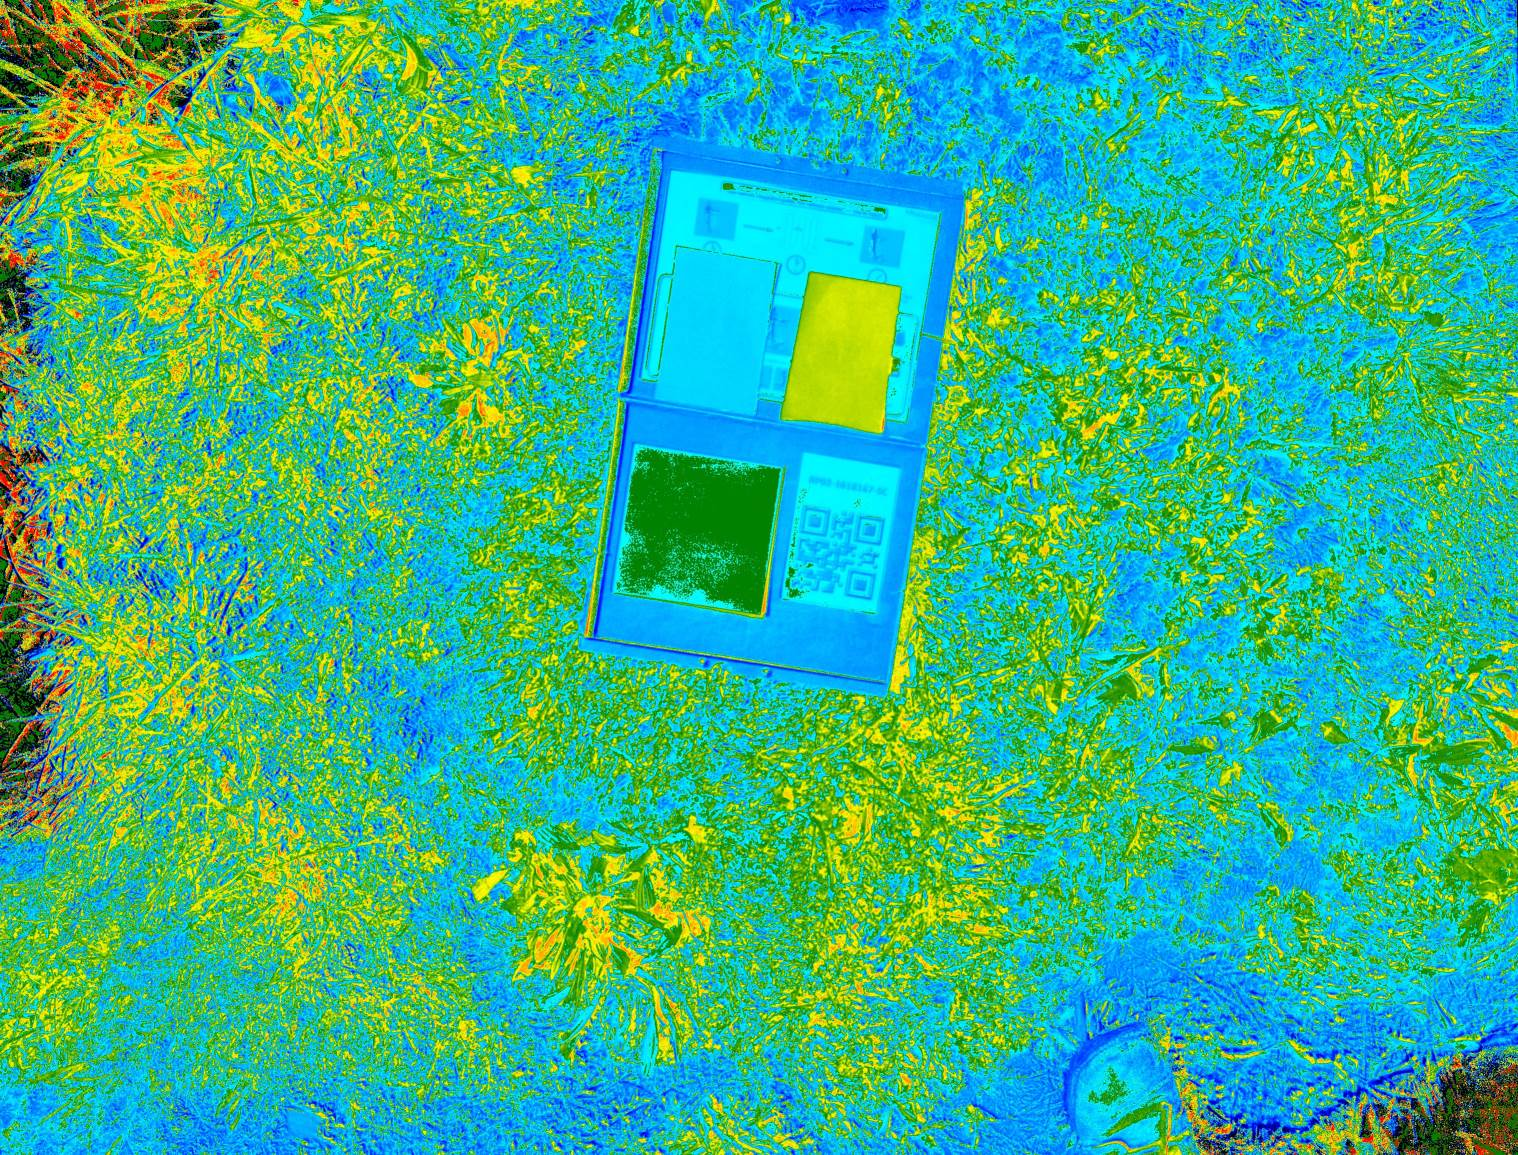
\includegraphics[scale=0.17]{images/ndvi_cal.jpg}
\caption{Processed NDVI image}
\end{subfigure}
\caption{Calibration plate}
\label{fig:cal_plate}
\end{figure}